% Chapter 1

\chapter{Introducción general} % Main chapter title

\label{Chapter1} % For referencing the chapter elsewhere, use \ref{Chapter1} 
\label{IntroGeneral}
En este capítulo se presentan los principales tipos de paneles de mensajes variables, los motivos que condujeron al desarrollo de este trabajo y por último se explica el alcance y objetivos.
%----------------------------------------------------------------------------------------

% Define some commands to keep the formatting separated from the content 
\newcommand{\keyword}[1]{\textbf{#1}}
\newcommand{\tabhead}[1]{\textbf{#1}}
\newcommand{\code}[1]{\texttt{#1}}
\newcommand{\file}[1]{\texttt{\bfseries#1}}
\newcommand{\option}[1]{\texttt{\itshape#1}}
\newcommand{\grados}{$^{\circ}$}

%----------------------------------------------------------------------------------------

%\section{Introducción}

%----------------------------------------------------------------------------------------
\section{Panel de mensajes variables}

Los paneles de mensajes variables son señales de tránsito diseñadas para alertar o informar al usuario de la carretera. El panel de mensajes variable puede mostrar pictogramas o mensajes escritos, las imágenes en pantalla pueden ser estáticas, parpadeantes o realizar efectos. %\agregar referencia bibl. 
%\https://es.wikipedia.org/wiki/Panel_de_mensajes_variables#cite_note-1

\subsection{Panel de mensajes variables permanente}

Los paneles de mensajes variables permanentes generalmente se montan en estructuras aéreas que abarcan la carretera, en voladizo sobre una parte de la carretera, o fuera de la carretera, y se utilizan para influir en los automovilistas con propósitos de control de tránsito. Sus mensajes pueden cambiarse manual, mecánica o electro-mecánicamente para proporcionar a los automovilistas información sobre congestión del tráfico, accidentes de tráfico, operaciones de mantenimiento, condiciones climáticas adversas, condiciones de la carretera, eventos organizados u otras características de la carretera. Un beneficio de los paneles de mensajes variables permanentes es que pueden soportar un mayor tiempo, desplegar mensajes más detallados y permitir un mayor tiempo de exposición para que los automovilistas comprendan los mensajes antes de llegar a un punto de decisión.En la figura[\ref{fig:vmsp}] se muestra una pantalla de mensajes variables permanentes.


\begin{figure}[hptb]
	\centering
	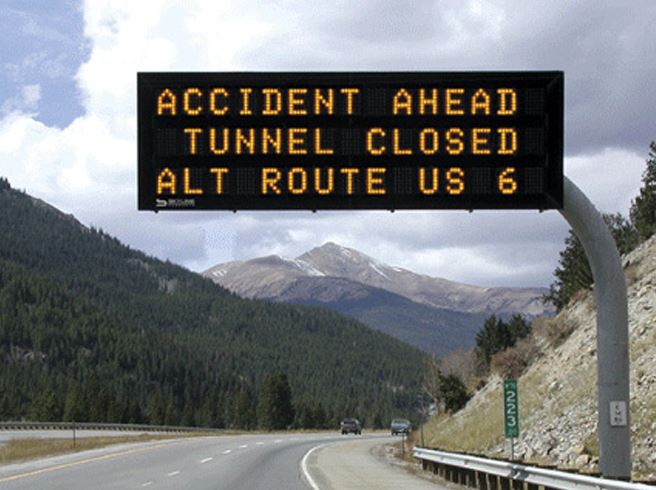
\includegraphics[scale=0.6]{../Figures/vmspermanente.jpg} 
	\caption{Panel de mensajes variables permanente.}
	\label{fig:vmsp}
\end{figure}
%----------------------------------------------------------------------------------------




\subsection{Panel de mensajes variables móvil}

Los paneles de mensajes variable móvil suelen estar montados en un remolque con paneles solares, son de fácil movimiento y pueden ser colocados cerca del punto de decisión. Los paneles de mensajes variable móviles se  pueden cambiar de forma manual, mecánica o por medios electromecánicos para proporcionar a los automovilistas información sobre la congestión del tráfico, los accidentes de tráfico, operaciones de mantenimiento, condiciones climáticas adversas, condiciones de la carretera, eventos organizados u otros características de la carretera. Un beneficio de los paneles de mensajes variables móviles es la posibilidad de ubicación en puntos estratégicos.En la figura[\ref{fig:vmsm}] se muestra una pantalla de mensajes variables móvil.

\begin{figure}[hptb]
	\centering
	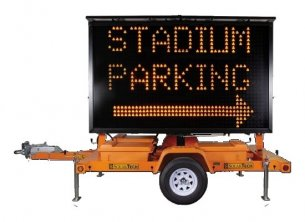
\includegraphics[scale=1]{../Figures/vmsmovil.jpg} 
	\caption{Panel de mensajes variables móvil.}
	\label{fig:vmsm}
\end{figure}
%/ https://www.enterpriseflasher.com/assets/images/solartech-1364402479.jpg


\subsection{Panel de mensajes variables montado en camión}

Los Paneles de mensajes variables montados en camión son generalmente unidades pequeñas montadas en o cerca de la parte trasera de un camión. Ellos generalmente tienen espacio para mensajes y tamaños de fuente limitados. Las limitaciones de sus mensajes suelen resultar en el uso de gráficos como flechas para mejorar la comprensión del conductor.

\begin{figure}[hptb]
	\centering
	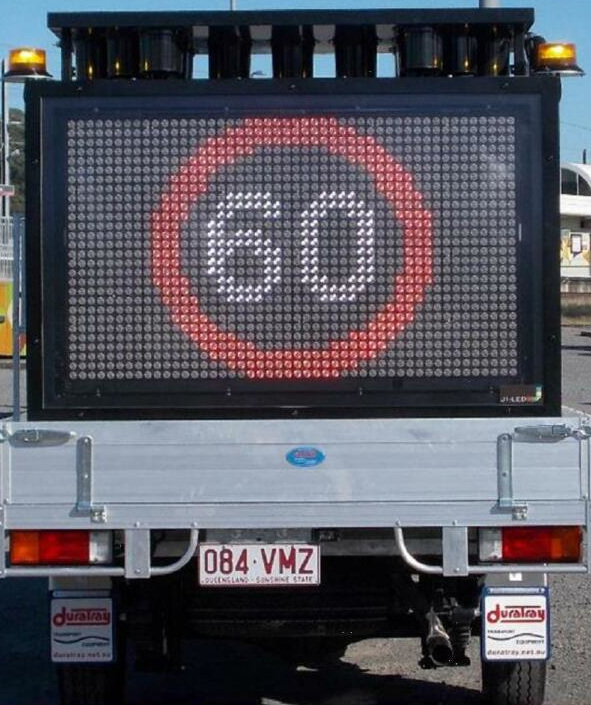
\includegraphics[scale=1]{../Figures/vmstruck.png} 
	\caption{Panel de mensajes variables montado en camión.}
	\label{fig:vmsc}
\end{figure}
%/ https://www.mobilesystems.co.nz/vdb/image/i2123


\subsection{Propósito del proyecto}
El propósito de este proyecto es desarrollar una pantalla gigante full color led. Se espera que el desarrollo de este nuevo producto diversifique el portafolio de productos viales que ya posee la empresa.
\subsection{Alcance del proyecto}
El presente proyecto incluye:

\begin{itemize}
\item Desarrollo de prototipo usando la board DE1-SOC.
\item Desarrollo de hardware para control.
\item Desarrollo de hardware matrices de leds.
\item Desarrollo de firmware usando linux embebido.
\item Desarrollo de una gpu que maneje las matrices de leds con FPGA.
\end{itemize}

El presente proyecto no incluye:

 \begin{itemize}
\item La interfaz gráfica para el cargado remoto de la imágenes.
\item La aplicación para cargar imágenes local.
\item Diseño de ventilación o mecánica de armado.

\end{itemize}




